\chapter{Background}
\section{Julia}

\subsection{Language Overview}
The goal of Julia is to solve the aforementioned two-language problem for scientific computing \cite{julia_intro}. The designers provide a language that can be used to easily express complex mathematical formulas and that produces fast low-level machine code to be used on processors. This low-level code is of a similar calibre to code generated by statically typed languages like C, in which it is more difficult to express the same mathematical formulas.

The design features that make Julia the language of choice for this project are:

\begin{itemize}
    \item Dataflow type inference.
    \item Multiple dispatch for method specialization.
    \item Meta-programming features for generating code.
    %\item Existing mathematical libraries that have been optimized to work with Julia.
\end{itemize}

\pagebreak

\subsubsection{Dataflow Type Inference}
Julia is a relatively easy language to pick up owing to its high-level nature and similarities to scientific computing languages like MATLAB and Python's Numpy. Julia does not require the declaration of static types for variables used within code. The following are implementations of a simple power function in C++ and Julia:

%caption={Basic power function in C++},
%captionpos=b, 
%label={code:cpow}

%caption={Basic power function in Julia followed by terminal output when compiled function is called.},
%captionpos=b, 
%label={code:jpow}]

%julia> jpow(2,3)
%8

\begin{figure}[htb!]
    \begin{subfigure}{0.48\textwidth}
\begin{lstlisting}[language=C]
//basic power function
int cpow(int x,int n) {
    int i;
    int result = 1;

    for (i = 0; i < n; ++i)
        result *= x;
    return(result);
}
\end{lstlisting}
    \caption{C++}
    \label{code:cpow}
    \end{subfigure}%
    \hfill
    \begin{subfigure}{0.48\textwidth}
\begin{lstlisting}
#basic power function
function jpow(x, n) 
    r = 1
        while n > 0
                n -= 1
                r *= x
        end
        return r
end
\end{lstlisting}
    \caption{Julia}
    \label{code:jpow}
    \end{subfigure}
    \caption{Basic power functions.}
\label{code:powfuncs}
\end{figure}

Code Snippet \ref{code:cpow} shows static typing. All variables must be declared before they are used and all types must be included in these declarations. This includes the inputs to the function. For a more complex function, it can be difficult and time consuming to select the most optimal type for high performing code.

With Julia, a layer of complexity is removed for the user. The types are not required for the code to successfully compile. In other languages (e.g. Python, MATLAB), this hampers performance as the compiler has to add in additional type checks to make sure that the correct code is used for the unknown data type. The dataflow type inference algorithm in Julia is able to define types automatically before the compilation has finished, reducing the amount of branching and redundant code run during run-time \footnote{If type inference is impossible for a variable, Julia uses a run-time library to manage any dynamic type changes at the cost of performance.}.

The type inference is done as a series of compiler passes that use any known type information about variables. If there are no explicit declarations, as in Code Snippet  \ref{code:jpow}, the compiler will make assumptions. For example, when the function is called, it will be provided with two input arguments:

\begin{center}
\code{jpow(2, 3)}    
\end{center}

Nowhere are the types of 2 and 3 declared, but the compiler assumes they are integer literals (since they do not contain a decimal point) meaning that the compiler will make them 64 bit integers. From the relation between \code{r} and \code{x}, it can be assumed that they are of the same type. This fully resolves the types for the function. Code that has manual type declarations will generally lead to more performant native machine code but, in many cases, this can be done in a different development stage to algorithm prototyping.
%as dynamic allocation and generalised, memory intensive types would be avoided. The compiler is able to use the sets of type information to narrow down abstract types, this results in the native code using quicker access stack memory to store values. For example, fixed array types are inferred instead of abstract vector types with variable size. There is less memory and overhead associated with the fixed type.

%The type inference forms a powerful combination with multiple dispatch. 

\pagebreak

\subsubsection{Multiple Dispatch}
Multiple dispatch is the process in which the compiler and/or run-time environment chooses a version of a function (method) that has been written and optimised with specific types as input. As with type inference, static dispatch occurs at compile time if and only if all types can be inferred for the appropriate method to be selected. This is similar to overloading functions in C++ but with less restrictions on input and return types for static dispatch. Dynamic dispatch occurs at run-time and chooses the correct method when the types are confirmed. A similar result can be obtained in C++ using virtual methods however these differ from overloading in their restrictions and syntax. The key benefit of Julia multiple dispatch is that it unifies the static and dynamic dispatch methods of languages like C++. This abstracts the different dispatch methods away from the user, disambiguates the method choices made by a program, and allows the creation of more readable code. Two methods for a generic function are written in \ref{code:mul_disp}. 

\begin{figure}[htb!]
\begin{lstlisting}[
caption={Two methods for a generic function \code{foo}. 
The code is compiled and the function name called in the terminal. The result displayed is the number of methods.},
captionpos=b, 
label={code:mul_disp}]
function foo(i::Int64)
        println("I use an Integer")
end

function foo(f::Float64)
        println("I use a Float")
end

julia> foo
foo (generic function with 2 methods)
\end{lstlisting}
\end{figure}


\begin{lstlisting}[
caption={Multiple dipatch example: function call results},
captionpos=b, 
label={code:mul_disp_out}]
julia> foo(1)
I use an Integer

julia> foo(1.0)
I use a Float
\end{lstlisting}

When the function is called in \ref{code:mul_disp_out} with an integer literal, the compiler chooses the method that takes an integer as input. The float method is chosen when a float literal is used in the function call.

Multiple dispatch allows users to write abstract functions that more closely resemble mathematical constructs and operations, but are optimised for the provided input types. The type inference narrows down the choice of types for variables with undeclared types, and then proceeds to choose the relevant optimised method for those types. This is not just the case for user-defined code, built-in operators like "+" use multiple dispatch to provide an abstraction for mathematical methods.

When provided with \code{$1 + 1$} Julia will infer the types as 64bit integers and choose a method of the "+" operator that can perform the operation on these types. If the user entered \code{[1, 2]$^T$ + [1, 0]$^T$} the types would be inferred as $2 * 1$ arrays of 64bit integers. Multiple dispatch the chooses "+" method (from the Julia LinearAlgebra package) that produces the optimal machine code for a vector addition. The user can then be as involved with type declaration as they feel comfortable, knowing that the compiler will generate high performing machine code by minimising branching and dynamic type checking overhead.

\pagebreak

\subsubsection{Meta-programming}
Meta-programming, in short, is the writing of code in a language that can create or transform existing code in the same language. Julia has a highly developed meta-programming structure that allows users to interact with and manipulate functions using the language itself \cite{julia_meta}.

Normal language users are primarily exposed to meta-programming via macros. Julia macros are code annotations prefixed by \code{@}. They are attached to variables and functions and can alter them or perform a separate function at the point of macro expansion within the compiler flow, before program run-time. Additional code is altered or inserted at this point to perform the function provided by the macro definition. An example is the assertion macro: \code{@assert \textit{condition}}. This expands to a conditional piece of code that returns nothing if the condition is true, and throws an error if false. This allows the user to write more readable code. 
%A macro example is \code{@code\_lowered function(x)}, this returns a snapshot of an intermediate representation of \code{function(x)} after some of the compilation stages have been completed. This is useful for seeing how code could be improved to take advantage of type inference and multiple dispatch.

\iffalse
if there's time, add a section about maths libraries
\fi
%\subsubsection{Existing Julia Packages}

\pagebreak 

\subsection{Compiler Flow}
\label{sec:compiler_flow}

Compilers transform user-defined code from higher level language to machine code that can be run on processors and other target devices. This is accomplished by performing compiler passes that parse source code to produce lowered code. These passes will strip away code abstractions, optimise high-level code structures for devices, and generate efficient and fast code to be run on target devices. To perform some of the passes, the source code is converted to a machine-independent data structure called the Intermediate Representation (IR). This IR is designed to be easier to optimise and translate than raw source code. 

\begin{figure}[tbh!]
    \centering
    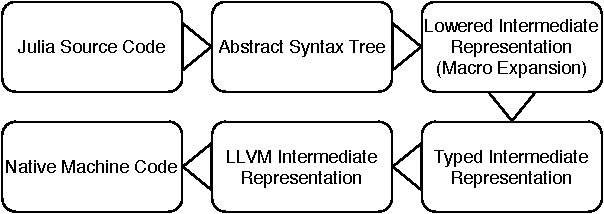
\includegraphics[width=0.6\textwidth]{Images/compiler_stage_simp.pdf}
    \caption{A high-level overview of the different forms produced during the stages of the Julia compiler. User defined source code is transformed into the specified form at each stage.}
    \label{fig:julia_compiler_flow_simp}
\end{figure}

Julia source code is lowered into the different forms in Figure \ref{fig:julia_compiler_flow_simp} by the compiler. The source code is parsed and converted to an Abstract Syntax Tree (AST). The AST represents the structure of the program in terms of expressions, function calls, and arguments, without explicit syntactical punctuation like \code{end} statements \cite{ASTImpl2003}. The punctuation information is contained within the tree structure of the AST. The AST then undergoes inital dataflow type inference and the macros are expanded to manipulate their code. This returns the lowered Julia IR, an example of which is given in Code Snippet \ref{code:jpow_lir} for the \code{jpow} method. The lowered IR is in Static Single Assignment (SSA) form \cite{eng_compiler}. This means that each variable on the left-hand side is only assigned in that one line. The flow of information through the IR is from top to bottom: sections of code are further organised into basic blocks. Between each basic block are explicit branching conditional statements or implicit fall-throughs that connect the basic blocks and dictate the control flow. 

\begin{lstlisting}[
caption={The CodeInfo object returned when applying the \code{code\_lowered} function to the simple \code{pow} function from \ref{code:jpow}. "n@\_5" is a slot variable used to store the loop integer condition.},
captionpos=b, 
label={code:jpow_lir}
]
julia> @code_lowered jpow(1,1)
CodeInfo(
    1 -      n@_5 = n@_3
    '--      r = 1
    2 - %3 = n@_5 > 0
    '--      goto #4 if not %3
    3 -      n@_5 = n@_5 - 1
    |        r = r * x
    '--      goto #2
    4 -      return r
)
\end{lstlisting}

\pagebreak

\begin{lstlisting}[
caption={The CodeInfo object generated from \code{code\_typed} on the \code{jpow} function \ref{code:jpow}. },
captionpos=b, 
label={code:jpow_tir}
]
julia> @code_typed jpow(1,1)
CodeInfo(
    1 -      nothing::Nothing
    2 - %2 = phi (#1 => 1, #3 => %7)::Int64
    |   %3 = phi (#1 => _3, #3 => %6)::Int64
    |   %4 = Base.slt_int(0, %3)::Bool
    '--      goto #4 if not %4
    3 - %6 = Base.sub_int(%3, 1)::Int64
    |   %7 = Base.mul_int(%2, x)::Int64
    '--      goto #2
    4 -      return %2
) => Int64
\end{lstlisting}

After the lowered IR, a data-flow type inference and method selection compiler pass is used to generate the typed IR, shown in Code Snippet \ref{code:jpow_tir} for the \code{jpow} method. The typed IR is in SSA form as well, and each line contains complete type information for the variables.

Slot variables in the lowered IR can represent function arguments or local variables that can be reassigned \cite{ci_doc}. Transitioning to the typed IR, the arguments remain slot variables but the local variables are replaced with a \code{PhiNode} structure. The \code{PhiNode} operations in a basic block evaluate based on the predecessors to the block, so they form part of the control flow of the program. The PhiNodes at lines 4 \& 5 in Code Snippet \ref{code:jpow_tir} determine what SSA variables 2 and 3 will equal, depending on the predecessor to basic block 2. This can be basic block 1 when the function starts or basic block 3 when the function loops around.

The compiler then transforms the typed IR into LLVM IR. The LLVM IR is a machine-independent SSA IR used to optimise code for different target machines and is typically used to produce fast native code for statically typed languages. Due to the complexity of the LLVM layer, the typed IR will be the focus of this project.

%\pagebreak

\subsection{Julia for GPUs \& Distributed Processors}
While many programs can run efficiently and quickly on single and multi-threaded processors, other programs that contain many nested loops, operate on large arrays of data or perform complex but repetitive operations have significant performance benefits when inputs can be split over the many processors in a GPU. %This provides hardware-based acceleration that has aided fields like medical physics \cite{gpu_acc}. 

A group of researchers have noted the two-language problem for GPUs and other hardware accelerators, and have created additions to Julia's compiler infrastructure to allow for the generation of efficient code to run on NVIDIA GPUs \cite{julia_gpu}. %Additional interfaces were introduced to extend the compiler to target NVIDIA GPUs. 
These additional interfaces enable sections of lowered code to be transformed to produce optimal LLVM IR for targeting GPUs. Many of the additions were able to rely on the meta-programming features of Julia to interact with LLVM IR. %The interfaces were designed to be extensible to other target devices to allow for future developers to implement LLVM-based compiler addtions. 
The performance was similar to specialised code benchmarks compiled with NVIDIA's own compiler. The compiler modifications have since be added to the main Julia codebase. 

The GPU project was extended to work with distributed processors \cite{julia_dist_plat}. In this case there were limited performance benefits due to the high communication overhead between processors. This project was successful in demonstrating the feasibility of programming generic array-based functions on GPUs and distributed processors with minimal knowledge of the target hardware. 
 
\section{High Level Synthesis}
\iffalse
- going to put in information about HLS
- hls intro paper
- legup papers
- nymble
- hatschet

- alaHLS?
\fi
As the complexity of programmable hardware increases, low-level logic needs to be abstracted to increase productivity of hardware design engineers. HDLs, like Verilog, abstract designs to Register Transfer Level (RTL) from lower-level, manually-routed functional blocks. HLS takes this a step further by using higher level languages, like C and C++, to generate synthesisable hardware. 

\subsection{Overview}
Traditionally, HLS starts with a high-level specification written in a subset of a higher level programming language \cite{hls_intro}. This is compiled to a lowered formal representation.  Standard compiler optimisations, like the removal of dead code and loop unrolling, are performed. 

\subsubsection{Formal Representation}
The formal representation exhibits data dependencies from the inputs, through intermediary variables and function calls to the outputs. It also exhibits control flow dependencies because the basic blocks of code will branch or loop. It is possible to strip the control flows away by unrolling loops, but this can often lead to excessive code repetition, to the point of being unfeasible for use in hardware generation. This is resolved by combining the dependency flows, representing them as a directed Control Data Flow Graph (CDFG). This graph can be used to extract potential parallelisms within and between basic blocks. The typical HLS flow needs to perform three main tasks when manipulating this graph: allocation, scheduling, and binding. These tasks are interdependent and have their own constraints on the hardware design produced.
 
\subsubsection{Allocation}
Allocation concerns the distribution of hardware resources to the functions described in the formal representation. These resources may be blocks of memory, functional units like multipliers, or linking components like buses. Allocation methods require constraints on resources, power consumption, and area. Functional block components are selected from a library with statistics about the power, resource usage, and delay. 

\subsubsection{Binding} 
All operations and variables must be bound to specific units within the FPGA architecture. This means choosing specific function blocks like adders and Block RAMs and assigning them to the scheduled operations, making sure that functional blocks are reused where possible. The transformed representation is then translated to an HDL for synthesis.

\pagebreak
 
\subsubsection{Scheduling}
Scheduling typically falls under two main categories: dynamic and static. Static scheduling assigns each operation within the CDFG a cycle count to operate on, making sure that data dependencies are maintained. Constraints on the static schedule are:
\begin{itemize}
    \item The duration of the functional blocks used for an operation.
    \item The order of dependent operations.
    \item The data dependencies across loops and branches.
\end{itemize}
Operations can be scheduled to happen in parallel if there's no data dependency, or can be chained together in a pipeline to feed through sequentially to make use of the benefits of FPGAs. The results of computing a static schedule produce a Finite State Machine that dictates the strict order of operations deduced from the control flow aspects of the CDFG.


In contrast, dynamic scheduling takes individual operations and maps them directly to functional operators with additional communication logic. This communication logic ensures the operators do not begin their computations until all input data is ready, allowing the operations to take place out of order while still preserving the dataflow dependencies through the generated hardware. There are benefits and disadvantages to both methods which will be further explored in the Analysis \& Design section. %TODO link or smth



\subsection{Existing Tools}
\subsubsection{Legup}
Legup \cite{legup_intro} generates hardware from C programs, converting the high-level code to a series of functionally equivalent blocks of hardware with additional control flow logic.
%hybrid soft processor and functional block architecture for implementation on FPGAs. The compiler chooses which sections of code should be "hardened" to functional blocks and which should remain as machine code to run on the soft processor. This allows a wider subset of C to be implemented within the full architecture. 
Legup makes use of the LLVM IR as the formal representation of the high-level code. Operations in this IR are simple enough to directly correspond to functional blocks, so are fed into static scheduling, allocation, and binding passes in the CDFG form. 

The passes are implemented separately so the algorithms used for each can be changed. Legup initially used ASAP scheduling - a very simple algorithm that just assigns clocks to each operation in order. In later work, Legup was compared to other HLS flows and improvements were made in execution time at the expense of higher energy usage for pure hardware flows.

\iffalse
- nymble for generating graphs

- similar flow and architecture to legup with the aim to include a larger subset of the c language
- be able to create complex hardware software interfaces automatically
- pieplining loop execution even with nested loops, exposing parallelism between basic blocks

- Nymble allows for fully shared memory space for processors and fpga fabric to communicate and share data

- key aspect is the adaptions for the Clang compiler to allow for custom directives to be used to alter the compiled LLVM
- this aids with generation of their CDFG
- they carried out work to compare the RTL generated and found that a pure DFG generated suboptimal code as it required more interfaces between functional blocks

- LLVm ir is static single assignment form meaning that variables are only occur on the left-hand side once and are not reassigned within basic blocks
- basic blocks are collections of operations that can be performed sequentially and do not required branching or looping, these are organsised between the control flow linking the basic blocks into a full program
- the linking of this forms the control flow graph
- nymble generates CDFG comprised of op nodes and edges that model dataflow to produce cdfg
- produce a graph for each loop determined by LLVM loop analysis
- calculate condition that controls execution, direct translation of special ir instructions
- phi nodes become MUXs, surrounding operations are transformed to have a predicate input and actual data value input from the branched nodes, used to join branched if else type statements
- explain what phi nodes are here???
- second instance of mux is used to model across loop instances

- since there will likely be nested loops, graphs are themselves nested and communication blocks are used to transfer data between them
- memory dependency edges are added between loops that require variable storage to compute
- load store and loop have additional predicates since they can take extra cycles 
- additional dependencies have to be considered when facotring in pipelined designs, memory dependencies working both ways

- hardware-specific optimisations done as well as standard machine-independent
- operator chaining, simple ops like adds shifts can be done within a cycle, heavily relies on accurate block models of timing, may differ if done extensively
- memory port multiplexing, having a static memory cache per instance of memory access and store would result in too many
- distributed caches reused for the differing GDFGs within the program
- some cdfg may be too large so require dist cache for reduced resources
- use of local memory, accesses usually stored on external ram but have support from using BRAMs to improve access times for smaller mem reqs
- benchmarked using CHstone suite - DSP to cryptography
\fi

\pagebreak

\subsubsection{Nymble}
The Nymble \cite{nymble_intro} tool uses a similar flow and architecture to Legup with the aim of including a larger subset of the C language. It is able to expose parallelisms between basic blocks, meaning loop execution can be pipelined even within nested loops. %Nymble uses a fully shared memory space for the soft processors and FPGA fabric to communicate and share data.

Work was carried out to compare the generated RTL and found that a pure DFG generated sub-optimal RTL, as more interfaces were required between functional blocks. %Nymble adapted 
Nymble instead generates a CDFG comprised of nodes containing operations and edges that model dataflow. The Clang compiler was adapted to introduce custom directives to alter the compiled LLVM to aid the generation of the CDFG. 

Separate graphs are produced for each loop determined by the LLVM loop analysis. The conditions that control execution are direct translations of special IR instructions. For example, the LLVM PhiNodes become multiplexers where the operations in preceding blocks are transformed to have a select line, as well as the data value output, connected to the node input. These are used to join branched if...else statements. %The second instance of multiplexer usage is used to bridge between loop iterations.

Nymble performs hardware-specific optimisations as well as standard machine-independent optimisations. These are:
\begin{itemize}
    \item Operator chaining to increase the number of functions within a cycle.
    \item Memory port multiplexing to reduce area usage.
    \item Reuse of distributed caches to reduce area usage.
    \item Exchange of slower external RAM modules for faster Block RAMs on the FPGA fabric.
\end{itemize}

%\pagebreak

\subsubsection{Dynamatics} %TODO - be nice to write a bit more about the lib, maybe diagram?

The Dynamatics \cite{dynamatics_p} tool flow performs dynamically scheduled HLS on a subset of the C language. As with Legup and Nymble, the flow starts by compiling the C source code using a standard Clang compiler to produce a formal representation of the code in LLVM. LLVM passes are then used to transform the code by reducing the branching and memory access complexity. The resultant simplified CDFG is then converted into an "Elastic Circuit". This circuit maps standard LLVM operations to their elastic components that are equipped with valid and ready signals so that the point at which they perform their operation is dependent on the valid/ready status of the predecessor and successor components. 

Once the CDFG has been converted to elastic components, additional control components are added to maintain the order of memory access operations, ensuring the data is read and stored at the correct point in the program flow. The components are listed as nodes and edges in a directed DOT graph format. The graph is then translated to VHDL using the list of nodes to instantiate the necessary elastic components, and the edges to link the valid/ready, data and control signals between each component.

The resulting hardware makes use of custom functional operations as well as existing IP from the Vivado HLS suite \cite{viv_hls}. The combined set of operations means that a larger subset of the C language can be covered by the Dynamatic tool.




















\iffalse
- hatschet for the scheduling algos

- a tool for flexible run time shceduling, the more difficult and time consuming aspect of the hls flow
- designs are often limited by the available resources, for larger applications things cannot be done in parallel so ops need to be scheduled to the same resource, introduces resource constraint scheduling
- the problem can be formulated as integer linear programming and solved with standard solvers
- run into time issues when the problem is large, require heuristics and more info from the user
- modulo scheduling - interleave the schedules of inner loops so that multiple iterations can be executed in a pipelined fashion

- differnet algos - asap scheduling is a simple sched that hatschet can shoose when minimal compilation time is required 
- it orders operations and loops as the operations occur in order

- modulo sdc - modulo system of difference constraints is a much more time consuming scheduling problem to solve but will produce a more optimal order of ops in less cycles

- if you have time talk about modulo sdc scheduling

\subsubsection{HatSchet}
The most time consuming aspect of the HLS flow is scheduling. HatSchet \cite{hatschet} is a tool for flexible run-time scheduling and can utilise different scheduling methods. Since designs are often limited by the available resources, operations in larger applications cannot be done in parallel so need to be scheduled to the same resource. The standard scheduling problem can be formulated as integer linear programming and solved with standard solvers. This can take too long for larger applications so heuristics and more detailed user information is used to bound the problem. 

In addition to ASAP scheduling there is modulo scheduling. The user is able to select which algorithm to use based on the length of time available for scheduling. The modulo system of difference constraints problem is a more time consuming scheduling problem to solve but will produce a more optimal order of operations in less cycles.
\fi